The following section will go in to in depth detail about the system and how to use it. This section of the user manual will show you how to perform actions throughout the application.There will also be sections on what to expect from each action. Certain troubleshooting sections will be referenced in this text and if you encounter any of these errors please refer to the troubleshooting section to try and solve the error.

\subsection{Starting the program}
The program will allow you to perform eye-tracking on different kinds of media. Different media can be recorded and so the program will allow for multiple recordings of the same or different media. The program allows you to create what is known as a eye-tracking recording project. This project is used to keep all the information of your recordings for a specific session. You can always return to the session and continue recording in that project which allows you to move between recording projects.\newline

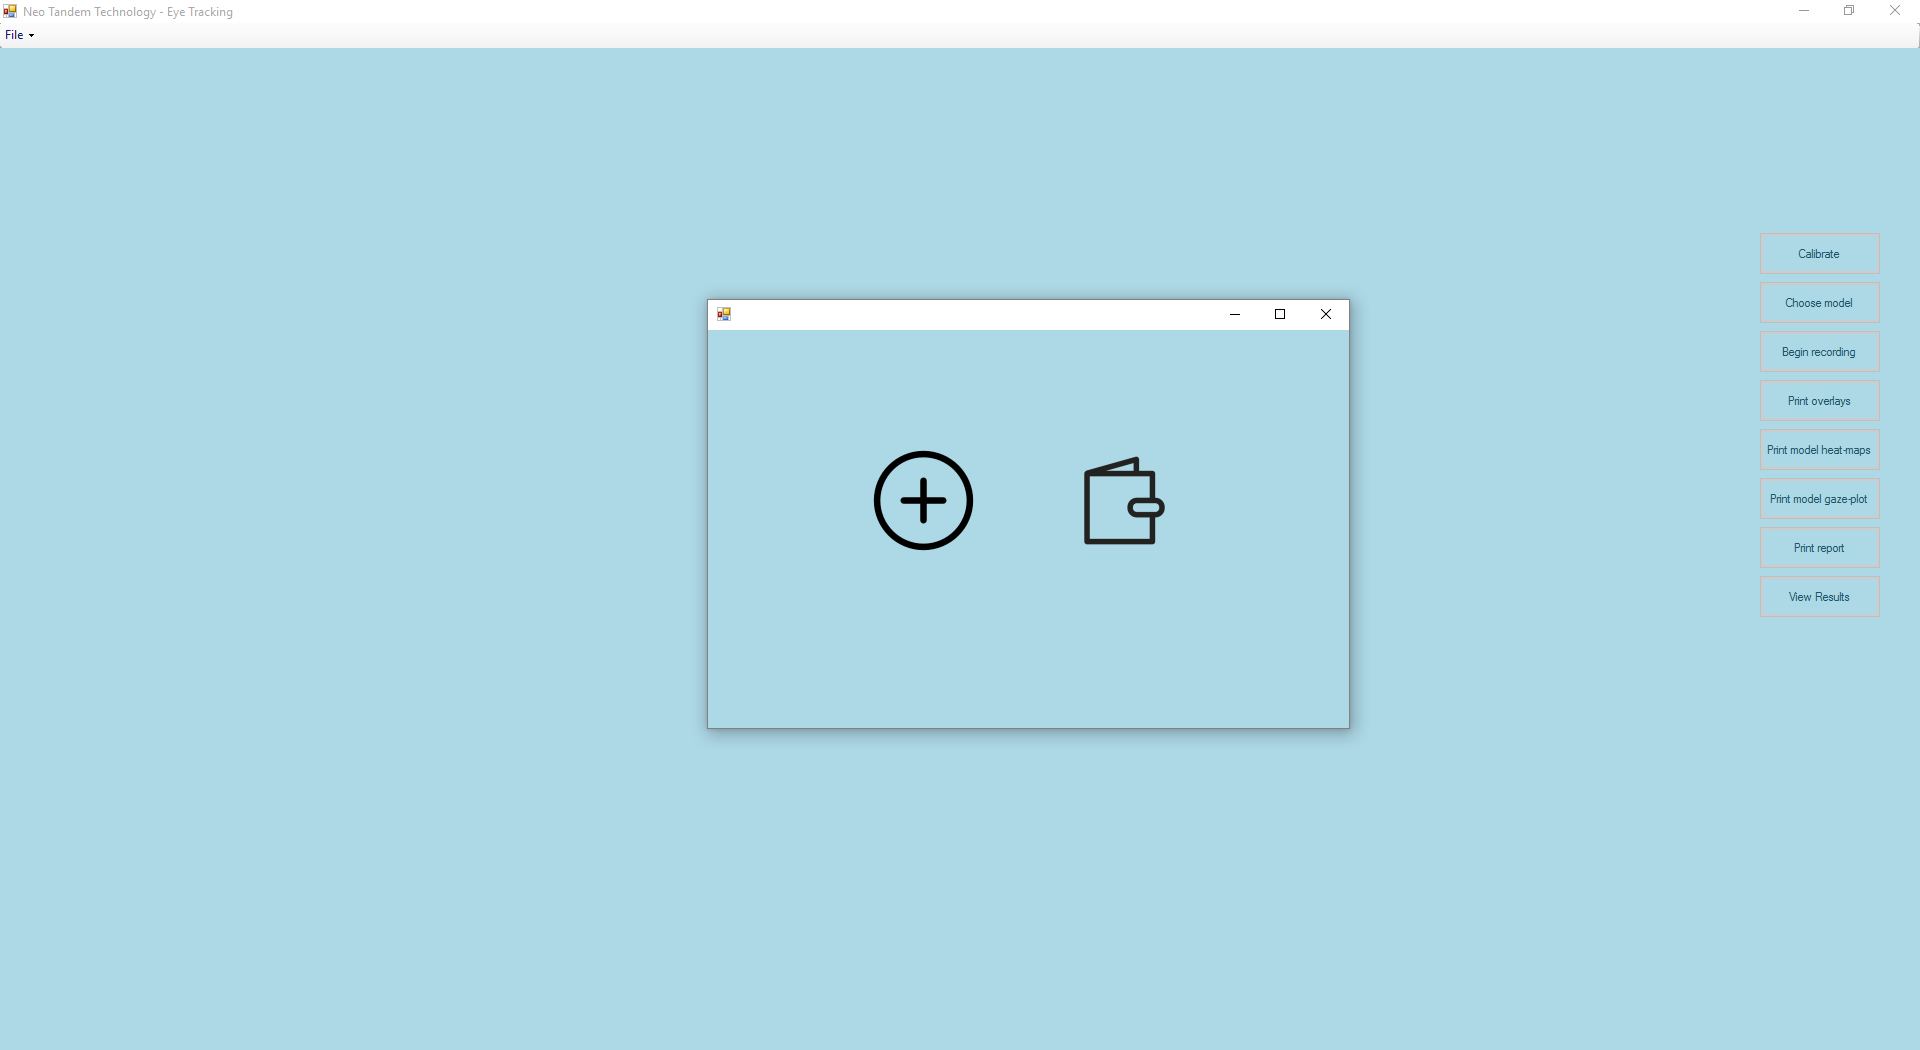
\includegraphics[width=400px,height=200px]{./Images/StartupPage.PNG}

When the user runs the Eye tracking software a form will appear. The form is split into two sections, start a new recording or to open a existing project.Below are the execution of both methods.

\subsubsection{Start a new project} 
To start a new project you will need to specify a name for the project and location to store all the files. A default name will be given to the project called "project". This will create 3 files and a series of folders in the location selected. The 3 files created are the .eye file which contains all the information about the recording project. This information is all that is needed to continue recordings. The two other files that are created are the settings files for general user settings and then settings for 3D recording.The folders that are created are just the folders for the recording data and the results. Once this all the folders are created then the program will proceed to the main menu.

		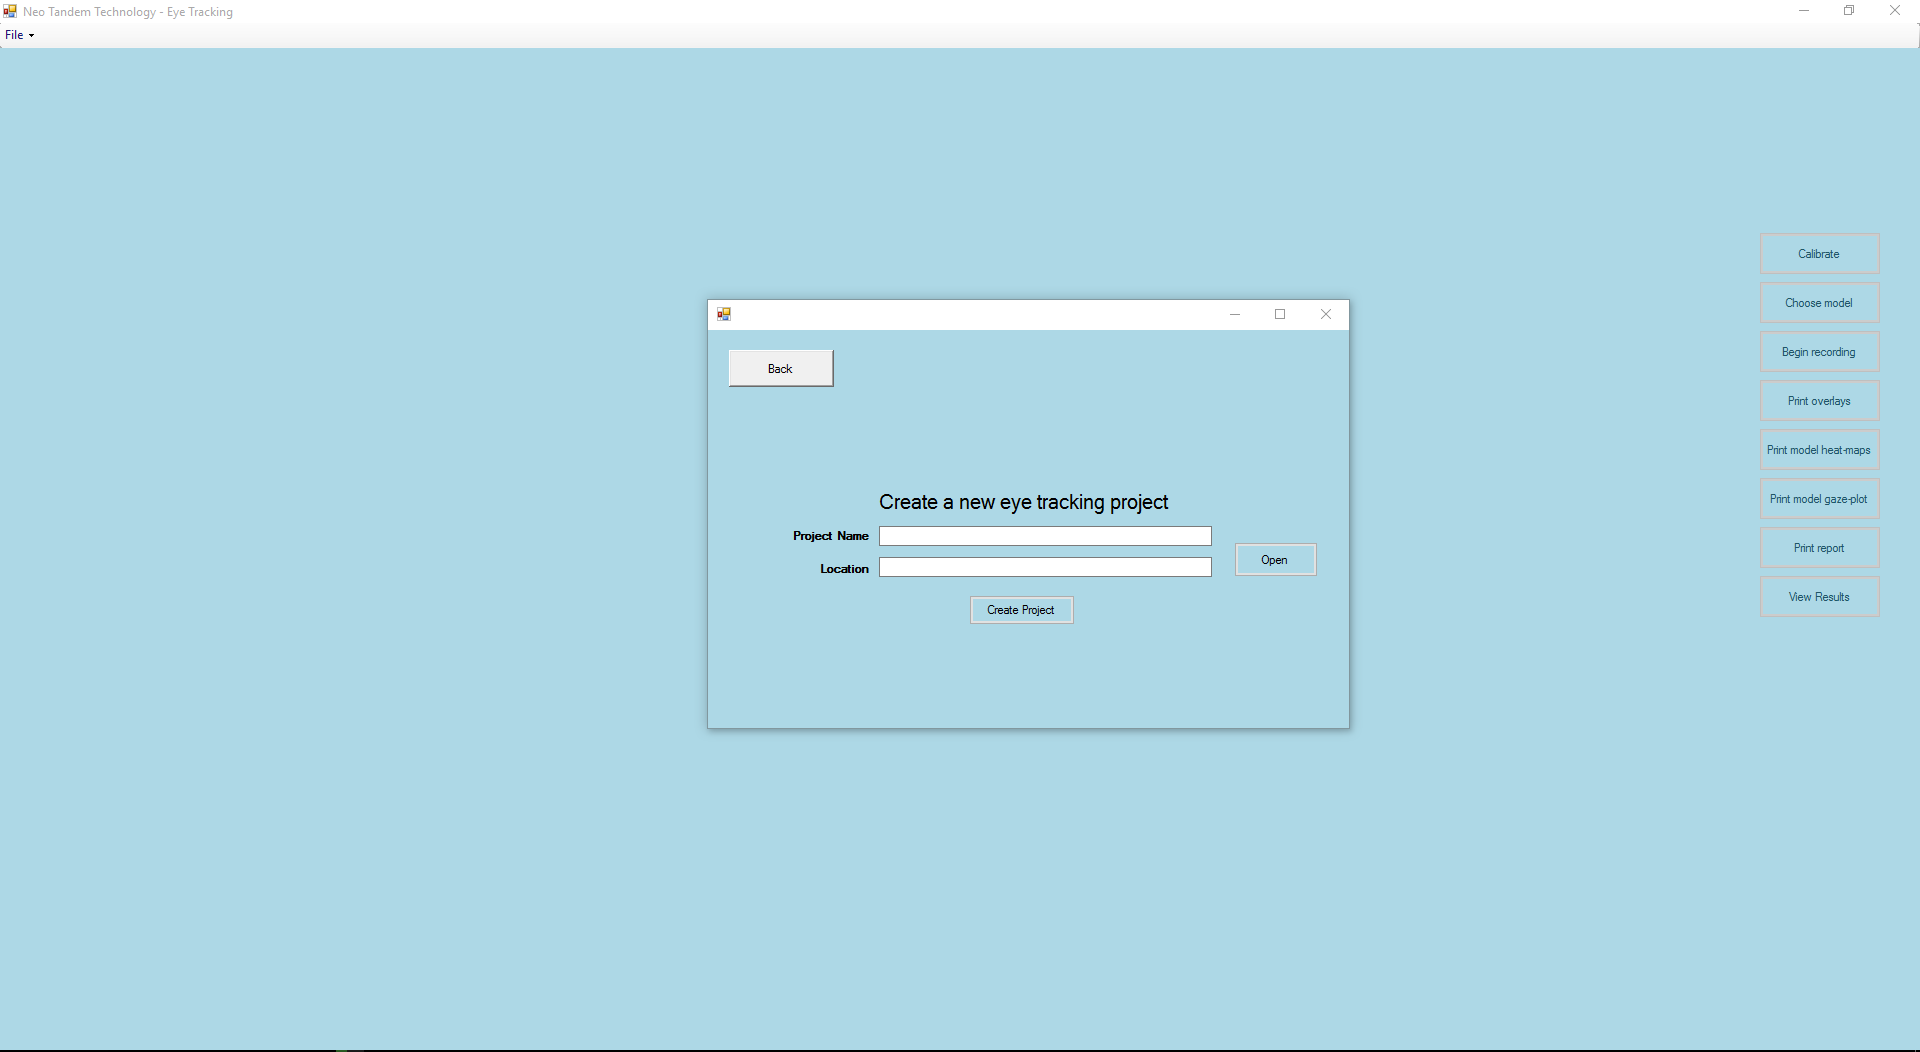
\includegraphics[scale=0.2, width=10cm, keepaspectratio]{./Images/NewProject.PNG}

\subsubsection{Open existing project} 
This will allow you to select an existing project and continue recording. Press the open button to select a file. The only file that will be accepted are ".eye" files. Once you select the file the settings are loaded up from the files and then the program moves to the main menu for you to continue recording.\\
		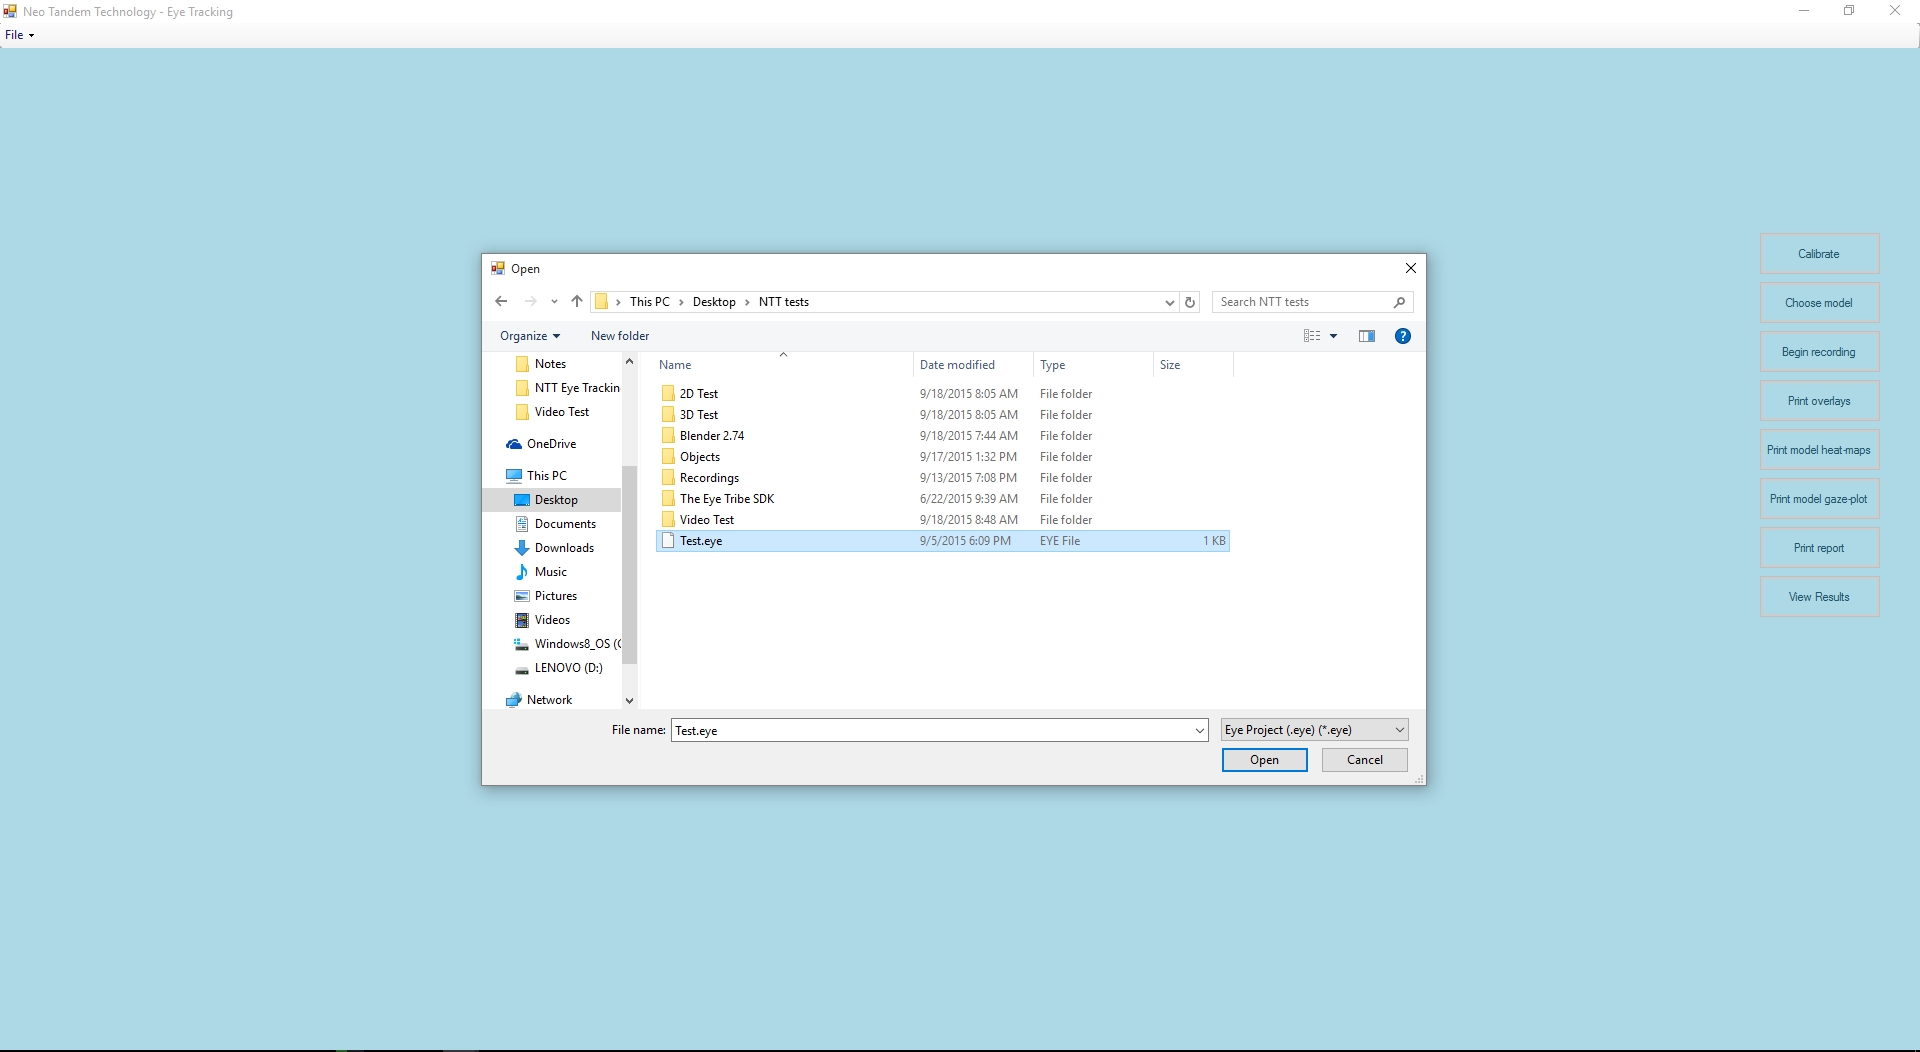
\includegraphics[scale=0.2, width=10cm, keepaspectratio]{./Images/OpenProject.PNG}\\
\iffalse
\subsection{Menu Screen}
The menu screen is where the program will allow the user to navigate through the entire application and perform all the tasks. The menu is divided into two sections. The calibration and the recording sections. The calibration button will navigate the user to the configurations page and will allow the user to calibrate The Eye Tribe camera. This will need to be done to ensure that the camera is recording the data accurately. There is more detail on the calibration below.

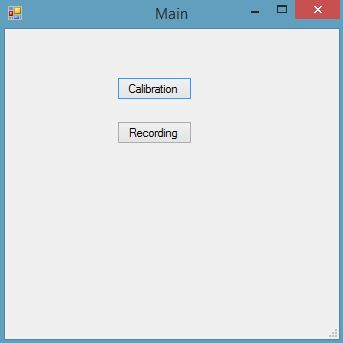
\includegraphics[width=400px,height=200px]{./Images/Mainpage.JPG}

The recording option will navigate to the recording set-up form which will be used to set up a recording. This will be discussed later on in the manual. While the menu screen offers navigation for the application it also provides a exit point for the application.This is where the the program is exited. This is achieved by pressing the red X in the top right corner of the form. This will safely end the program and ensure that nothing harms the computer.
\fi
\subsection{Calibration Screen}
When navigating to a recording screen there will be a button to navigate to the calibration screen.The calibration of The Eye Tribe camera is vital as this will ensure that the program will accurately create the heat maps for the media that has the eye tracking performed on it. This will also allow the user to configure the settings of the recording to their needs.The pressing of the calibration button will open the EyeTribeUIWin program which initiates the server and opens up the calibration. Use the calibration to calibrate the camera.Leave the server window open as this is what will transfer the data from the camera to the program. The server is connected to the internet so also ensure that there is a stable internet connection available. Once you have calibrated you may then proceed back to the menu screen and then start recording.

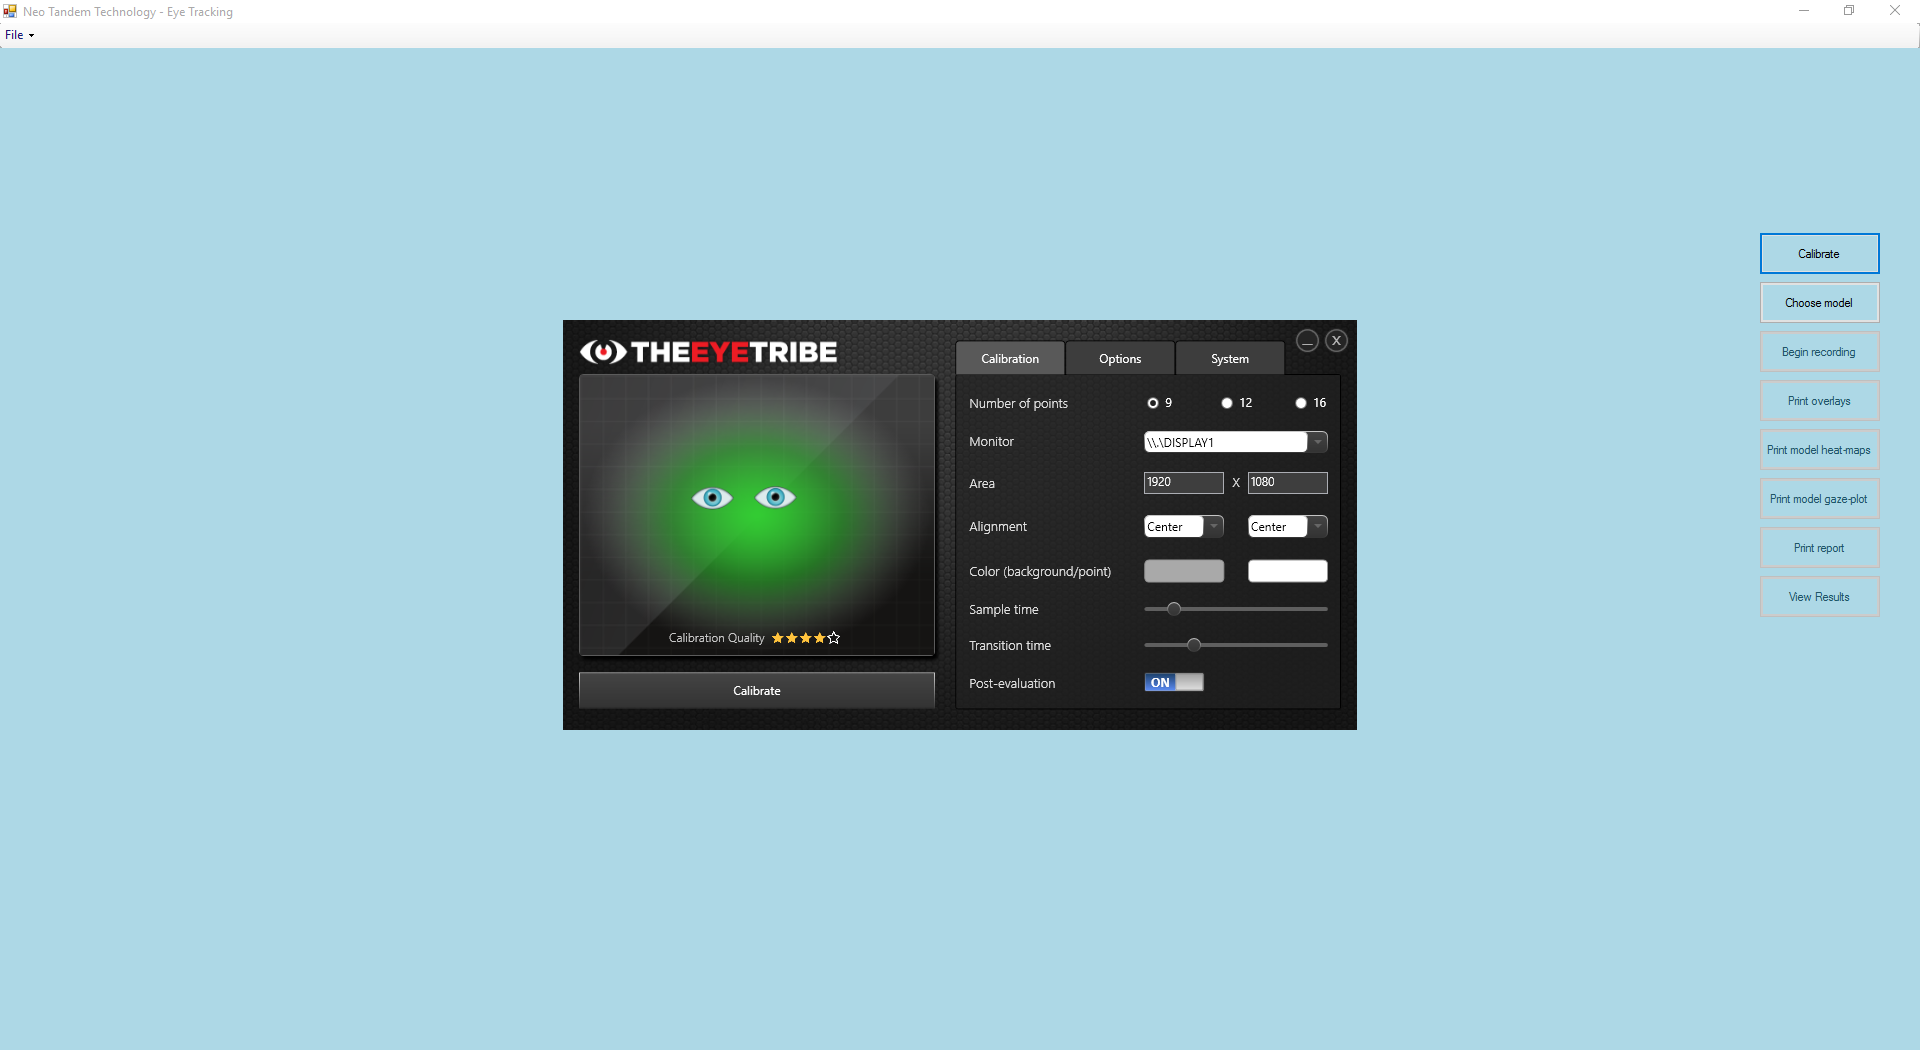
\includegraphics[width=400px,height=200px]{./Images/EyeCalibration.PNG}\\

The calibration will show the following if there is no camera detected\\


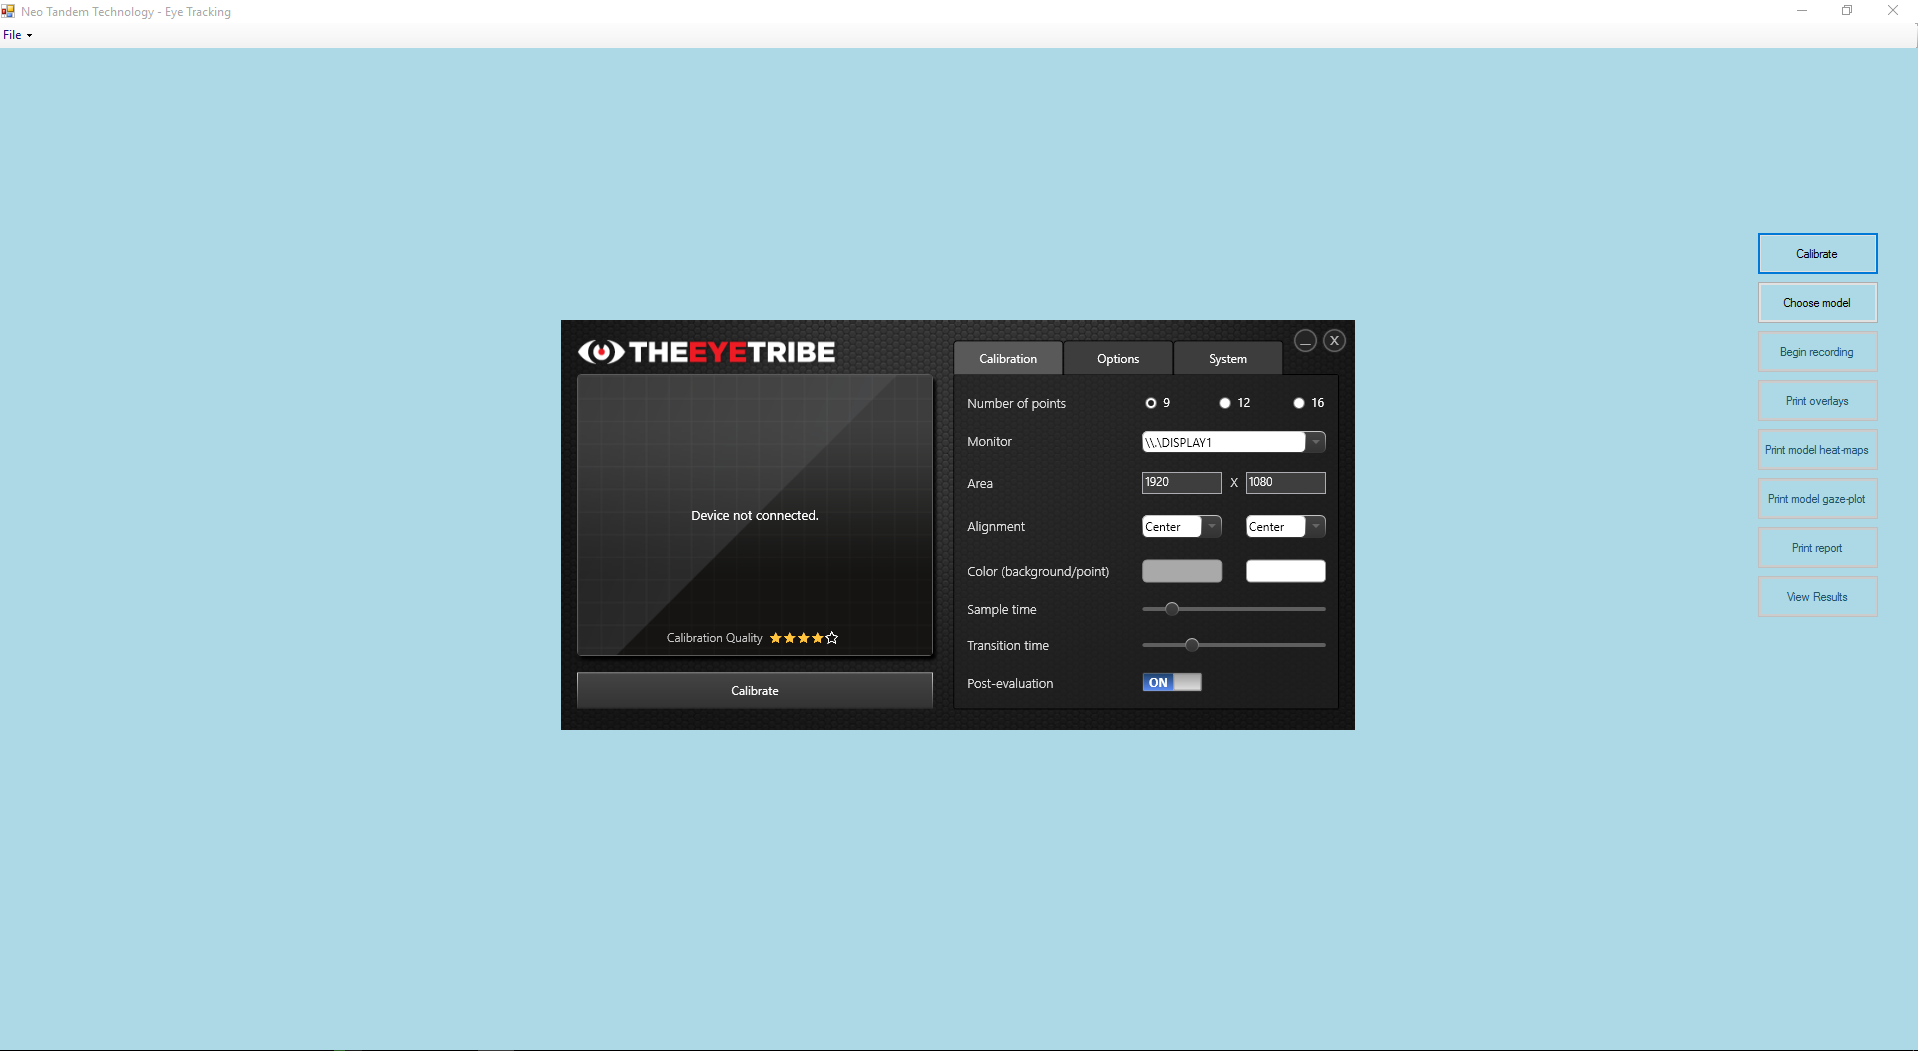
\includegraphics[width=400px,height=200px]{./Images/NoCameraCalibration.PNG}\\

The calibration will show the following if there is no eyes detected\\


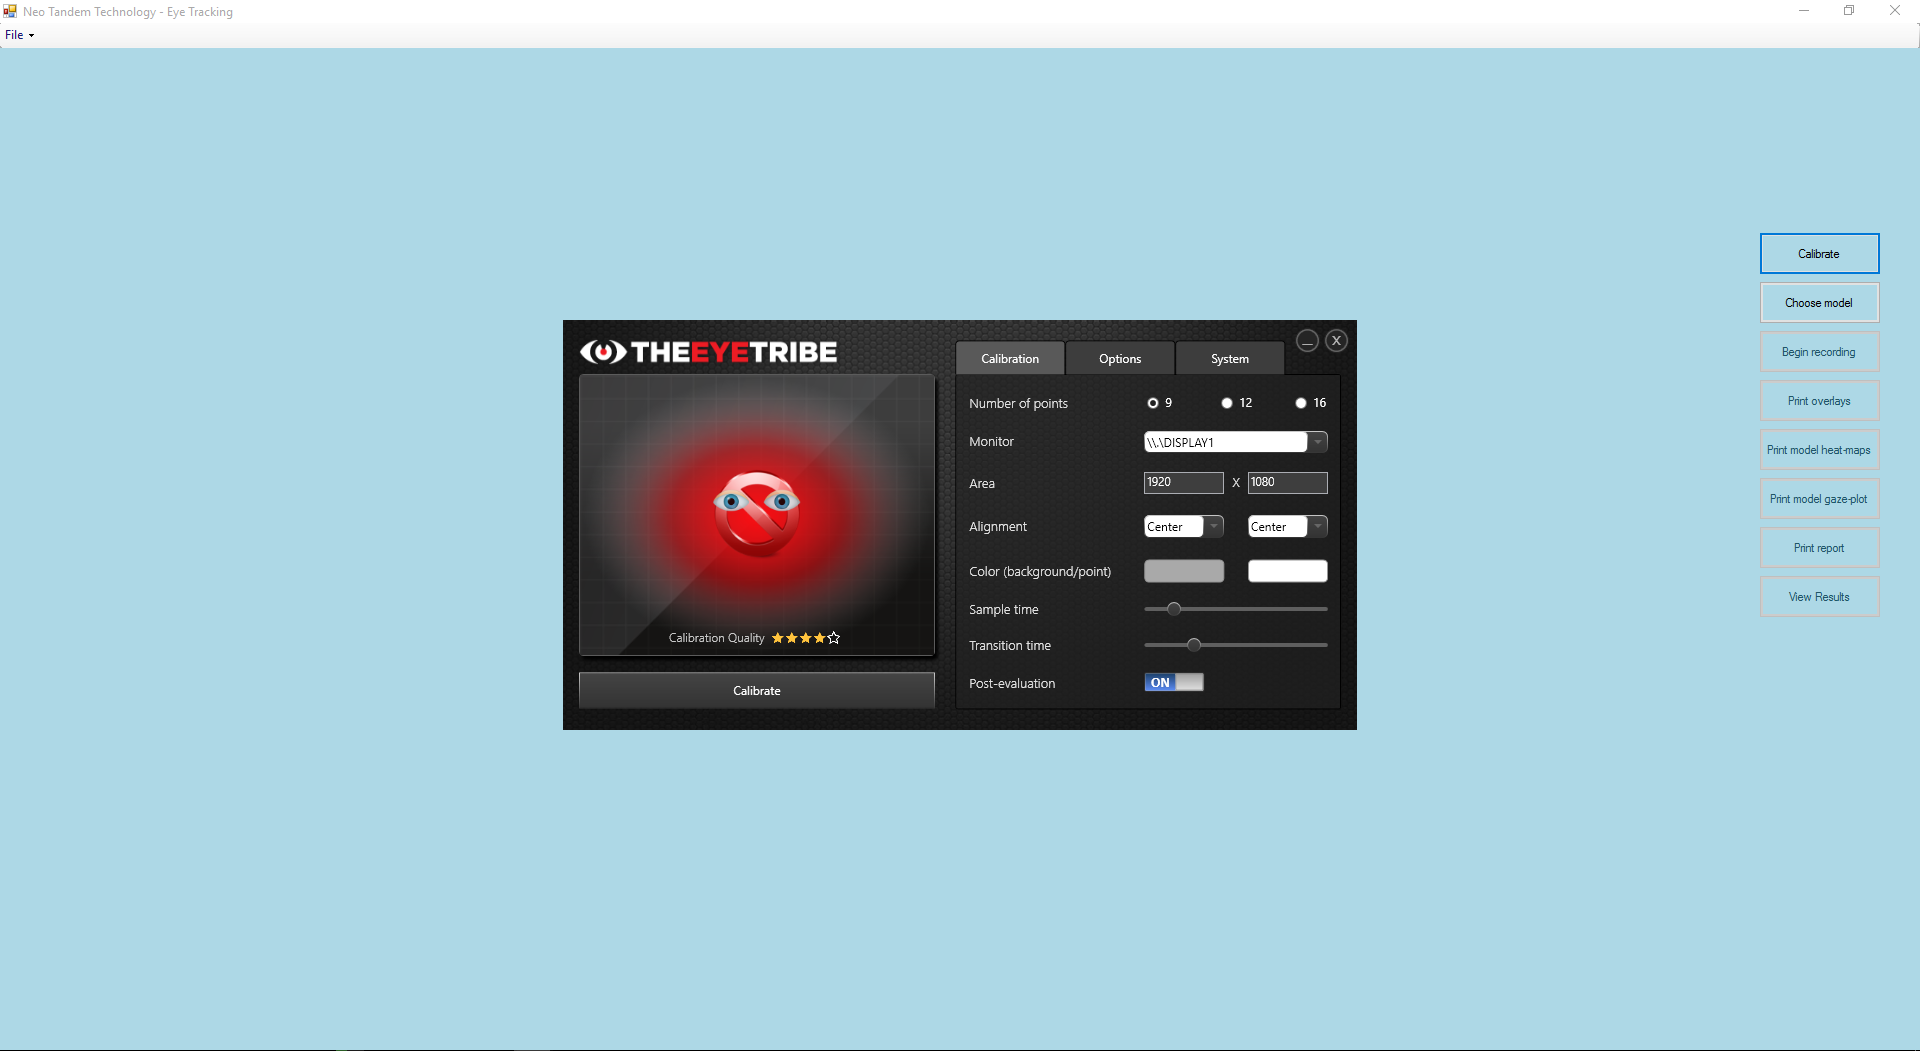
\includegraphics[width=400px,height=200px]{./Images/NoEyeCalibration.PNG}\\




\subsection{Recording Set-up Screen}
When you are done opening an existing project or starting a new one you will be navigated to this screen. This screen is used to set-up the recordings. This screen will allow you to do multiple recordings.These recordings are executed sequentially and can not be performed at the same time.
The application will be navigated to either of three screens: 2D recording screen, 3D recording screen or the Video recording screen. This navigation will be dependant on the options taken in the recording set-up.
You will also be allowed to name the recordings,this will create new folder in the recordings directory. The folder will be placed in the appropriate recording type sub-folder of the recordings folder. The folder will house all the information about the recordings such as eye-tracking data and also the resulting heat maps.

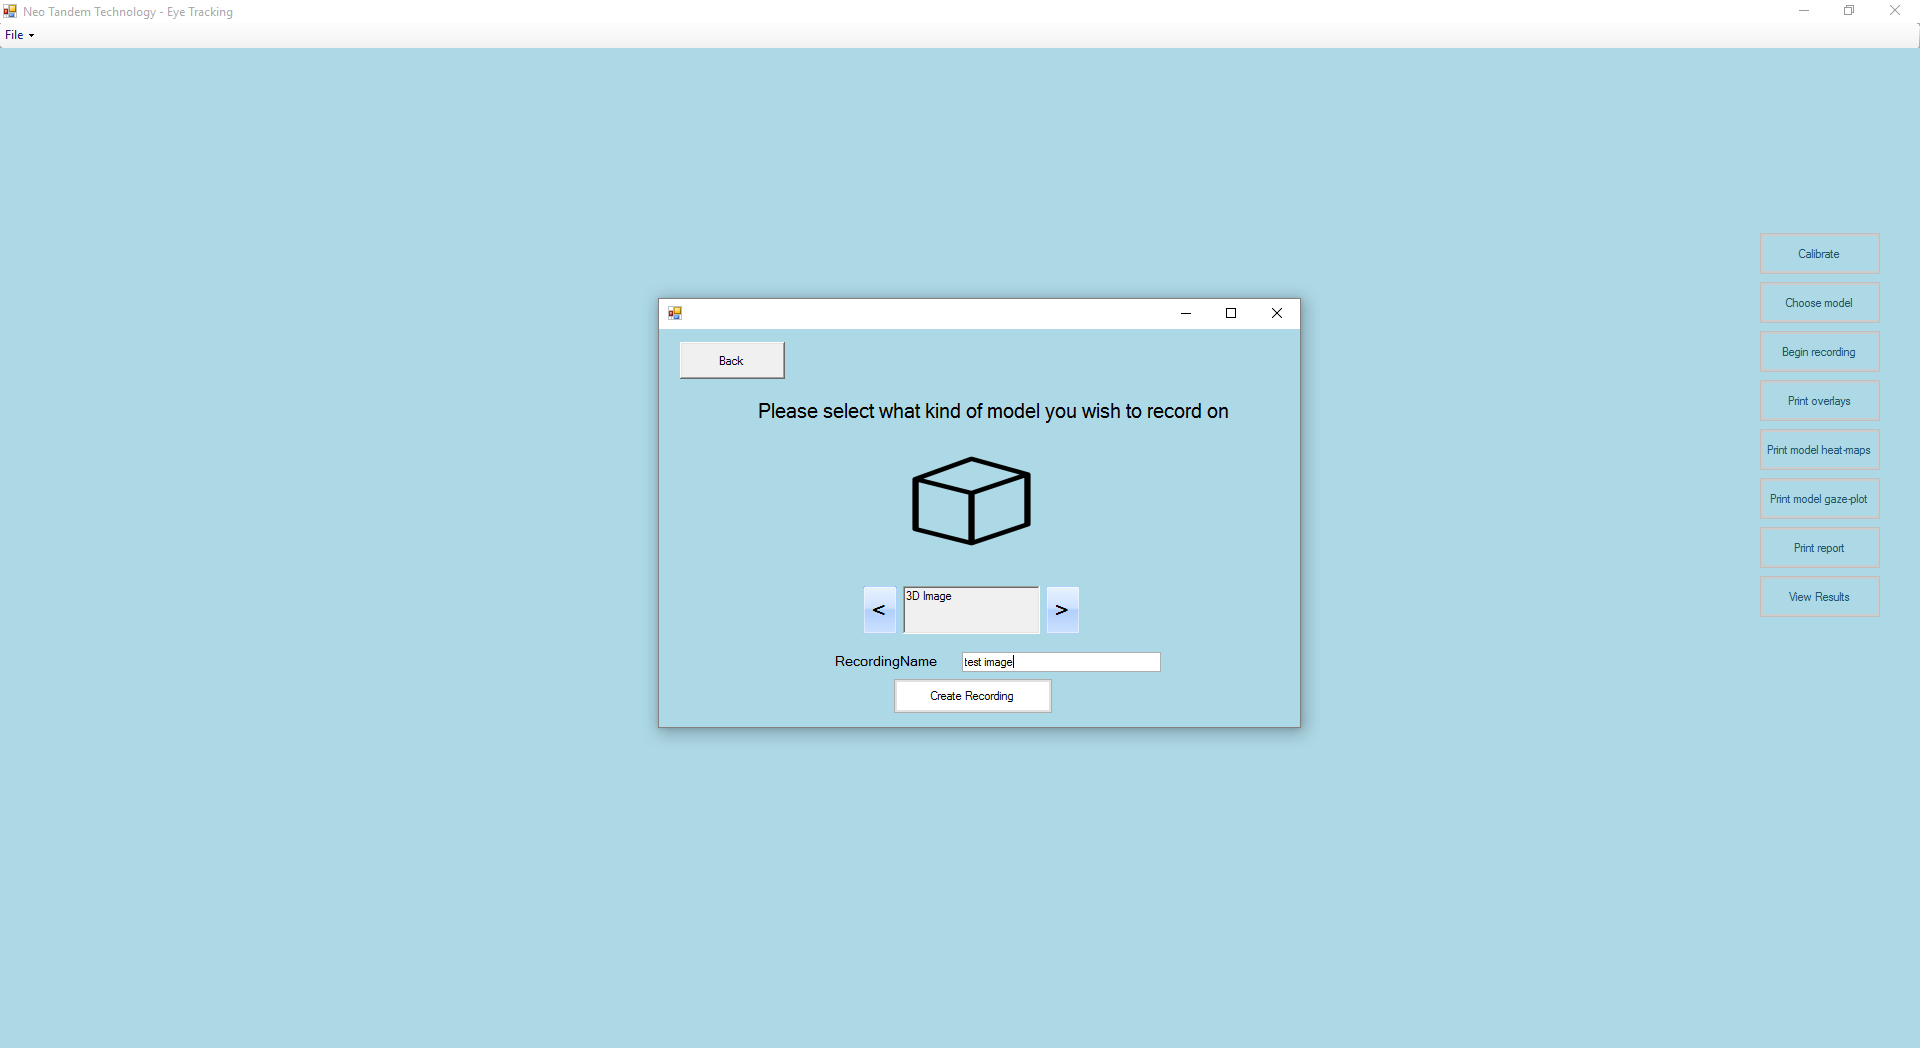
\includegraphics[width=400px,height=200px]{./Images/ModelSelect.PNG}

The screen has a text box for the user to enter the name of the recording. The name should contain only alpha numeric characters so that when the folder is created it will not fail. If it does not follow these rules then it will not be allowed to continue to the next section of the application. There is also a carousel that will cycle through various options to select what type of recording is needed to be performed. Once ready then press the start recording to proceed to the recording page.

\subsection{Choosing model}
The user must select the model they wish to do recording on by pressing the choose model option.This will open up a dialogue for the user to select their model.

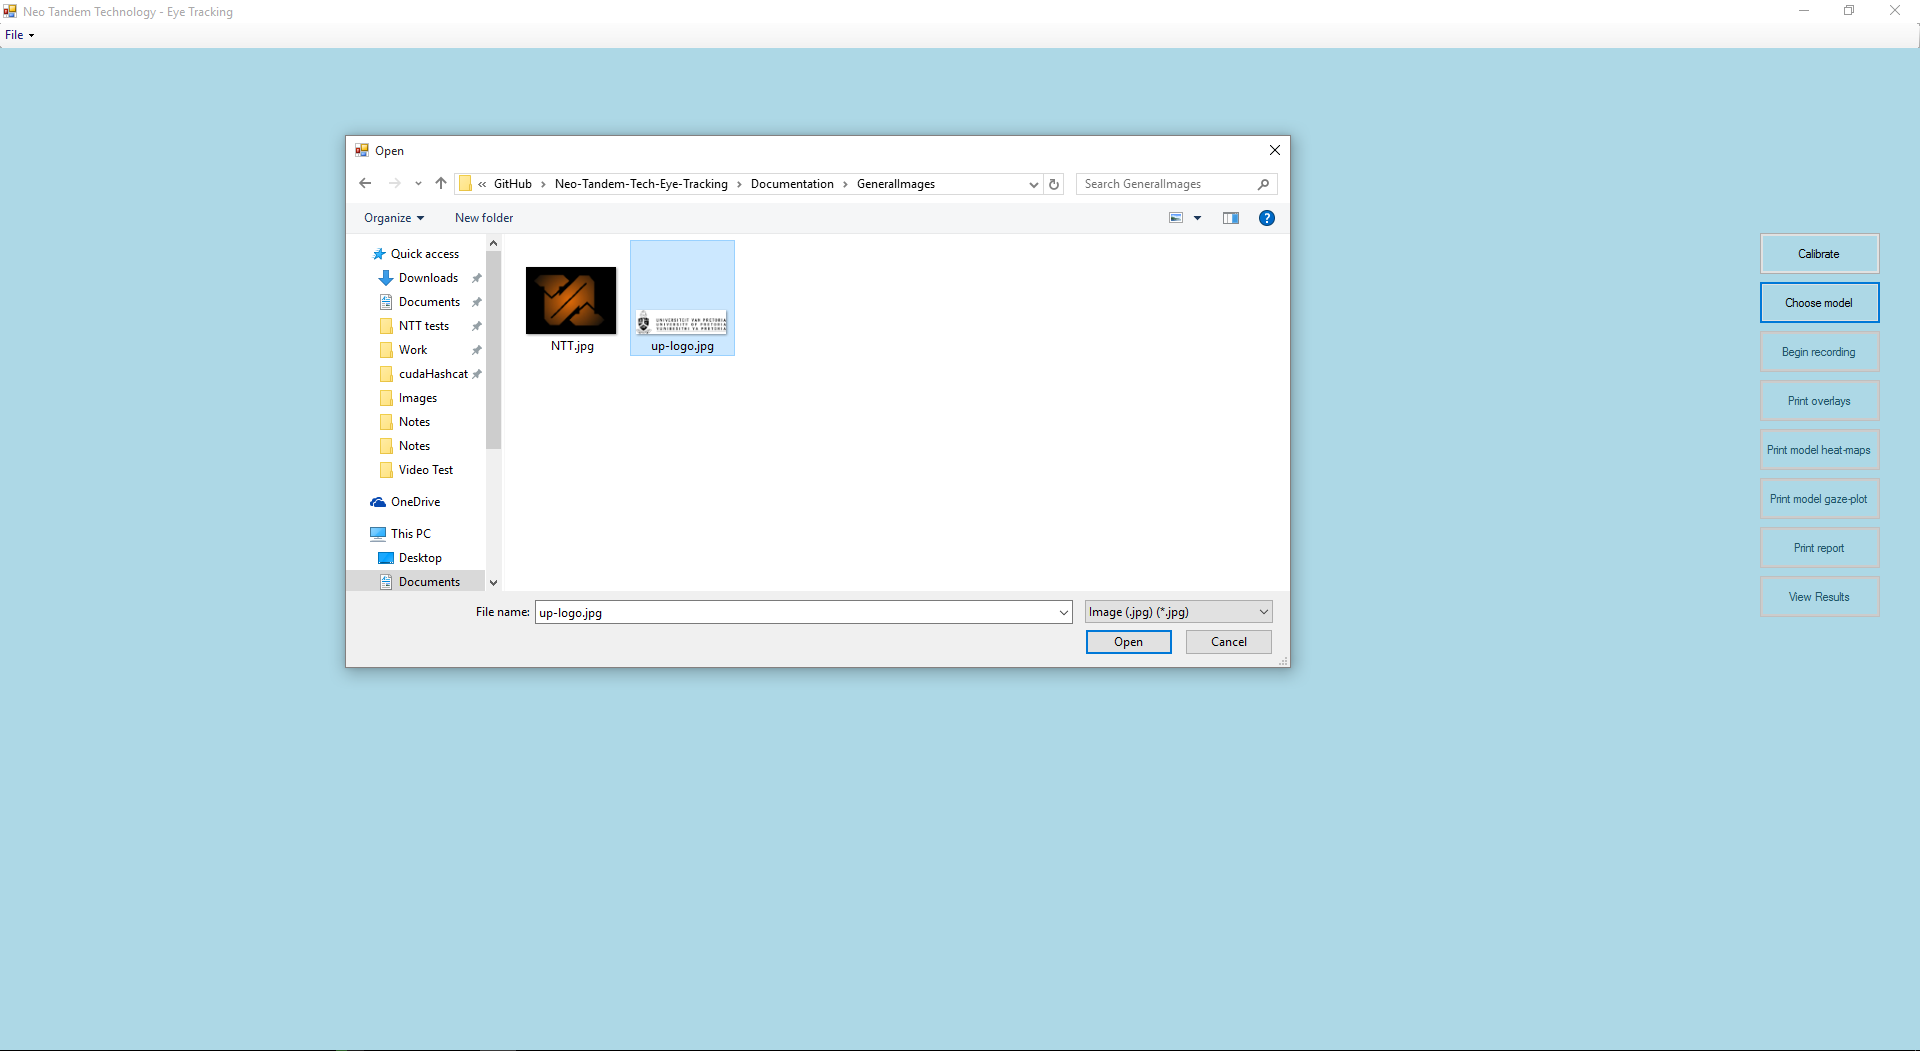
\includegraphics[width=400px,height=200px]{./Images/ChooseModel.PNG}

\subsection{Recording 2D model}
The 2D model recording form is navigated after the 2D model is selected in the recording set up. The page has a list of buttons that will perform all the tasks that need to be performed. The open model button when pressed,will allow the selection of a 2D model to be chosen. The 2D models are often just images and any image is allowed to be chosen. The quality of the image will improve the results from the eye tracking recording.The higher the image the more accurate the results will be. When an image is selected then the record button can be pressed. When the record button is pressed, the screen is filled with the image. The image is expanded to fit on the entire width and height of the image. The high image quality will provide a crisper and more clear image. The recording also starts ones the image is made full screen. During this process it is recommended that you move as little as possible as the data that is recorded could be tampered with. Once you are done with the recording press the Esc key. You are then able to find the results of the recording in the project location in the recordings folder and then in the folder with the models name as a folder. The folder will contain a copy of the image, a text file which contains all the recorded data and two images that have heat maps on them. The one heat map image is just the heat map while the other image is a heat map which then has the image that the recording was performed on. When you are done recording the data you can then exit the application or restart the recording. Restarting the recording will overwrite the data that was there. The exiting of the application is done through the pressing the red X in the top right corner of the form.\\

model displayed in the window and recording is ready.\\

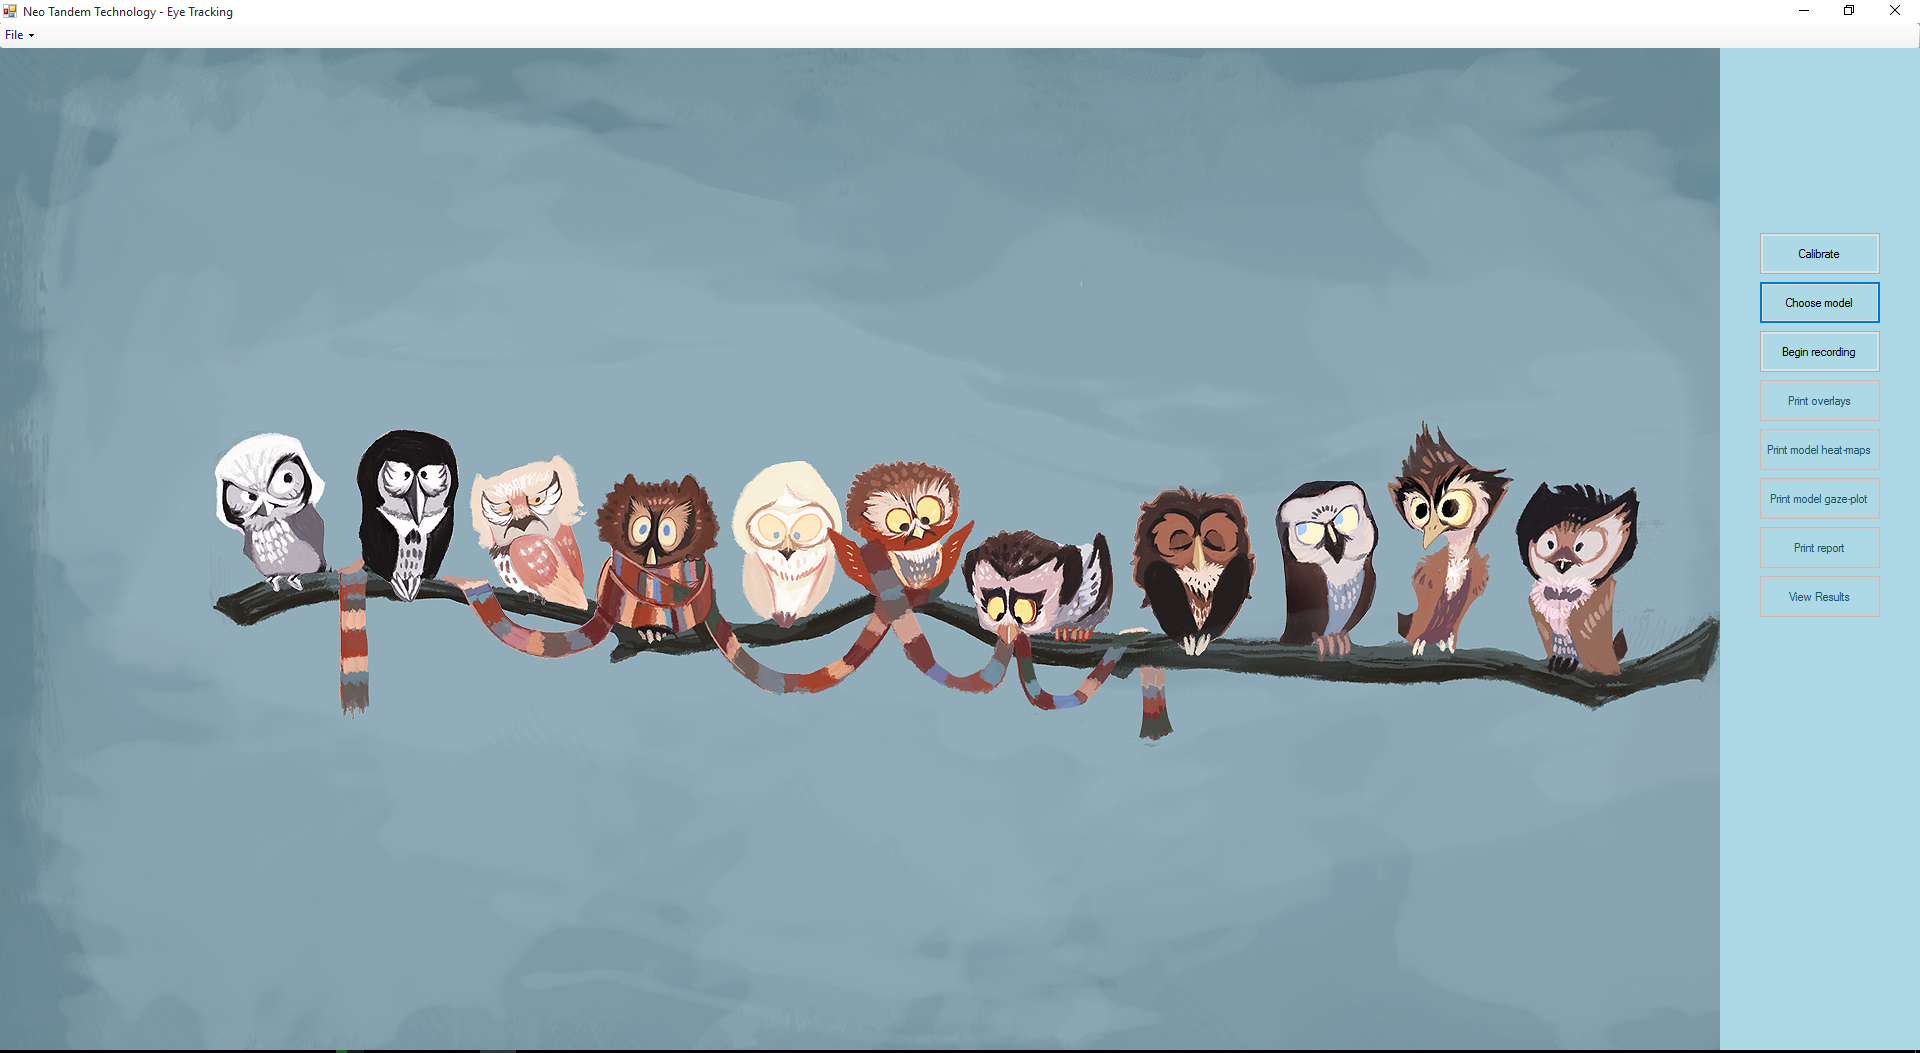
\includegraphics[width=400px,height=200px]{./Images/ModelPreview.PNG}\\

The recording occurring on a model,2D in this case.

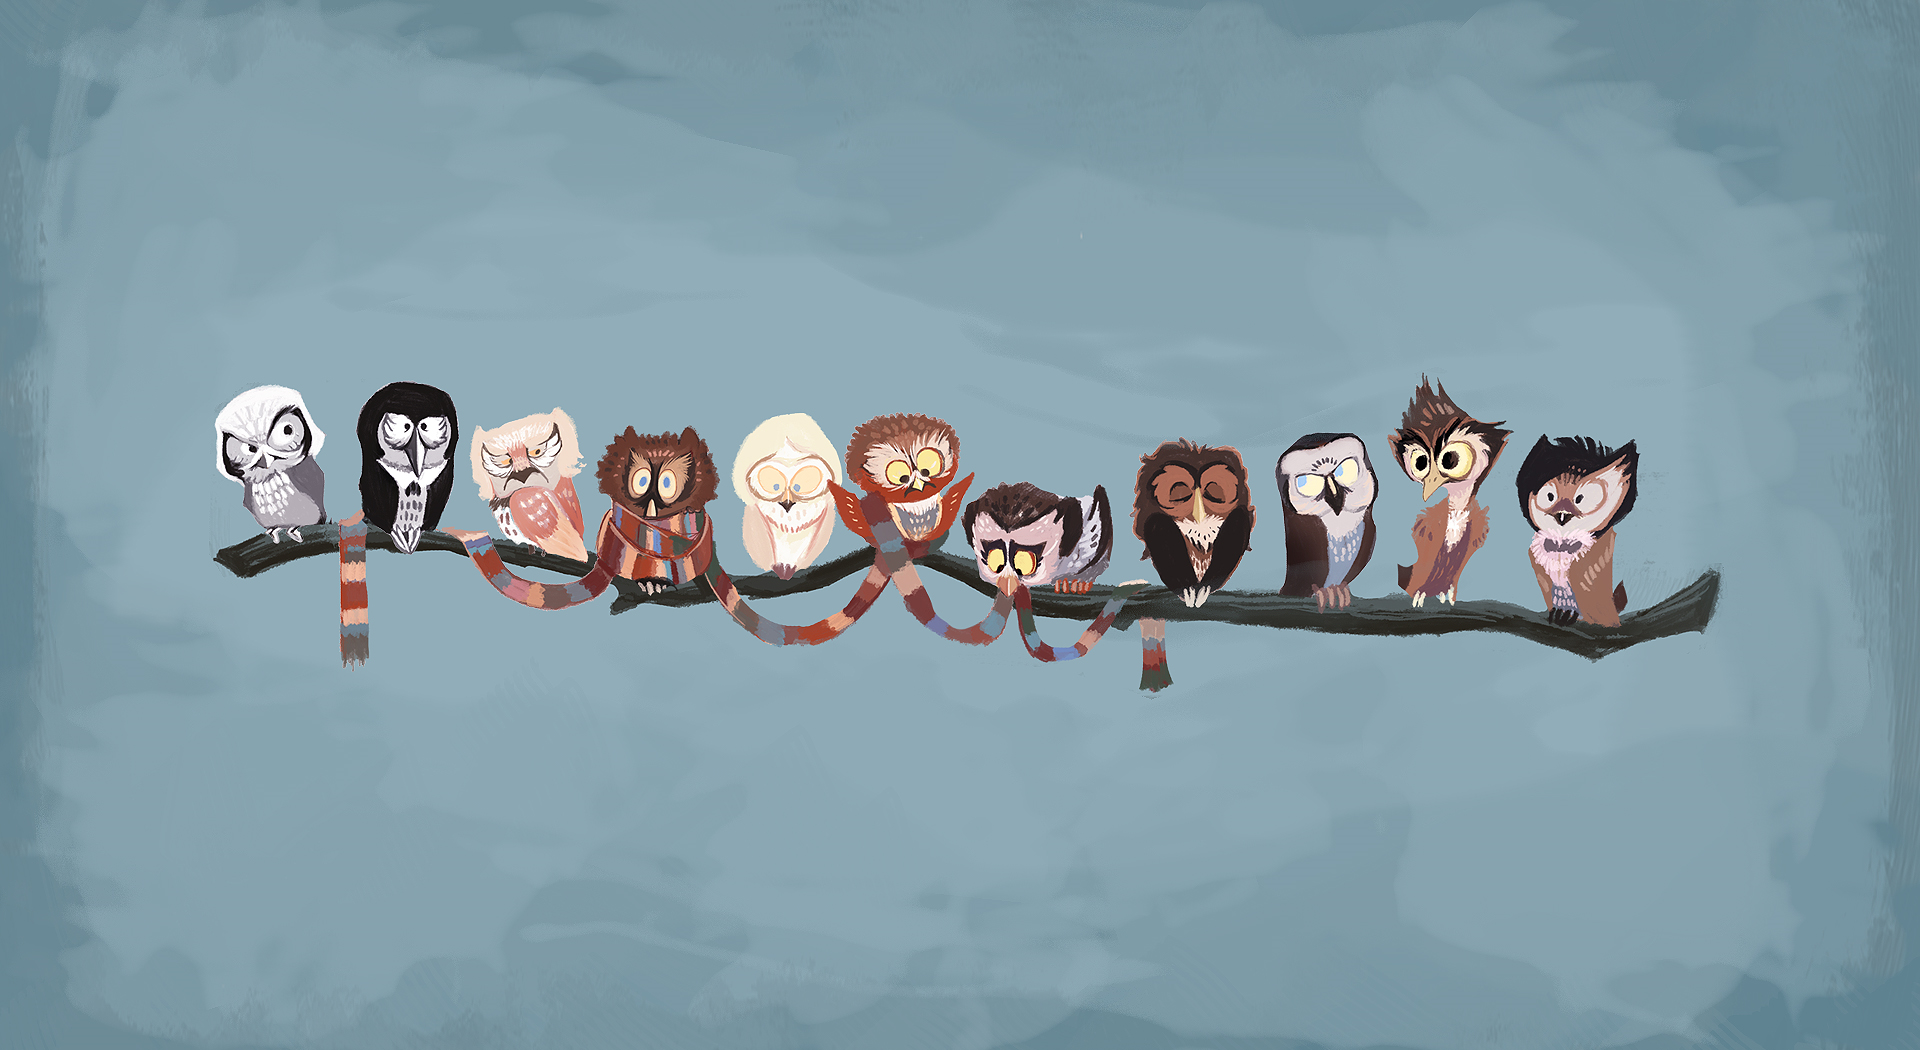
\includegraphics[width=400px,height=200px]{./Images/ModelDisplay.PNG}\\

\subsection{Recording 3D model}
The 3D model recording form is navigated after the 3D model is selected in the recording set-up. The page has a list of buttons that will perform all the tasks that need to be performed. The open model button when pressed,will allow the selection of a 3D model to be chosen. The 3D model will need to be in the format of a object file. These files have the extension ".obj". When an 3D model is selected then the record button can be pressed. When the record button is pressed. The 3D model then has snapshots taken and then a slide-show is created of the model and then is shown. The slide-show is expanded to fit on the entire width and height of the screen. The recording also starts once the slide-show starts the is made full-screen. During this process it is recommended that you move as little as possible as the data that is recorded could be tampered with. The recording process will end when all the slide-show images have been shown. You are then able to find the results of the recording in the project location in the recordings folder and then in the folder with the models name as a folder. The folder will contain all the snapshots, a text file which contains all the recorded data and images that have heat maps for each snapshot on them. The one set of heat map images are just the heat maps for each snapshot. while the other image is a heat map which then has the models snapshot that the recording was performed on. When you are done recording the data you can then exit the application or restart the recording. Restarting the recording will overwrite the existing data that was there. The exiting of the application is done through the pressing the red X in the top right corner of the form.

\subsection{Recording 3D model flythrough}
The 3D model flythrough recording form is navigated after the 3D model is selected in the recording set-up. The page has a list of buttons that will perform all the tasks that need to be performed. The open model button when pressed,will allow the selection of a 3D model to be chosen. The 3D model will need to be in the format of a object file. These files have the extension ".obj". When an 3D model is selected then the record button can be pressed. When the record button is pressed. The 3D model then is rendered and then the user is placed inside of the model and is then free to roam the model using either the keyboard or a gamepad. The 3D render is expanded to fit on the entire width and height of the screen. The recording also starts once the 3D render starts the is made full-screen. During this process it is recommended that you move as little as possible as the data that is recorded could be tampered with. The recording process will end when all the slide-show images have been shown. You are then able to find the results of the recording in the project location in the recordings folder and then in the folder with the models name as a folder. The folder will contain a video of your recording, a text file which contains all the recorded data and video that has a heatmap overlayed. When you are done recording the data you can then exit the application or restart the recording. Restarting the recording will overwrite the existing data that was there. The exiting of the application is done through the pressing the red X in the top right corner of the form.

\subsection{Recording Video}
The video recording form is navigated after the video is selected in the recording set-up. The page has a list of buttons that will perform all the tasks that need to be performed. The open video button when pressed, will allow the selection of a video to be chosen. The video that is chosen needs to be a ".wmv" file as it uses and extension of the Windows Media player. The length of the length of the video can be any length but the longer the video is the longer it will take to be processed. When an video is selected then the record button can be pressed. When the record button is pressed, the screen is filled with the video and the video will then start playing. The video is expanded to fit on the entire width and height of the screen. The video is recommended to be a medium quality one as the video might show signs of pixelation during the playing. The recording also starts once the video is made full screen and begins to play. During this process it is recommended that you move as little as possible as the data that is recorded could be tampered with. The recording will end when the video has stopped playing. Once you are done with the recording process you are then able to find the results of the recording in the project location in the recordings folder and then in the folder with the models name as a folder. The folder will contain a copy of the image, a text file which contains all the recorded data and two videos that have heat maps on them. The one heat map video is just the heat map while the other image is a heat map which then has the video that the recording was performed on. The heat map will be populated as time goes by showing the most looked at on the model. When you are done recording the data you can then exit the application or restart the recording. Restarting the recording will overwrite the data  that was there. The exiting of the application is done through the pressing the red X in the top right corner of the form.

\subsection{Report summary creation}
Once a recording has been completed on a model a statistical report is then generated with various details on the recording. The report is in a PDF format so a PDF reader such as Adobe reader is required to be installed on the computer to view the report. The report is located in the folder specified for the model.\\
The statistical report contains three pages. The first page is a cover page with a generic heading, the second page will contain data on the model. This information is just the basic meta data such as the models name, the models location and various other details about the model recorded.\\
The third and final page contains all the data for the recording that is then summarised. This data includes the number of points used and how many points where know as "lost points". Lost points are points that have been discarded as they are not in the bounds of the screen. These points have no impact on the creation of the heat-maps. The data also tracks the time of the recording based on the amount of points that are recorded.\\
The pdf also contains a grid of where the points are mapped on the grid. The grid is a three by three(3X3) grid and each sections represent a part of a screen. The grid is also used to determine a point of interest which is a section that has been looked at the most.\\
All this information is written to the PDF and then saved for later reading and quick view summary to easily and quickly see what happened in the recording. \\